\graphicspath{ {fig/} }
\begin{itemize}
\item{First example}

\tab The statistics shows that if a person is depressed and has anxiety , there is a 30 per cent change of it 
to commit suicide,where depression contributes 80% . Even if the person dosen't have those stimuly, it 
has a change of 5% to commit suicide.

\begin{center}
  	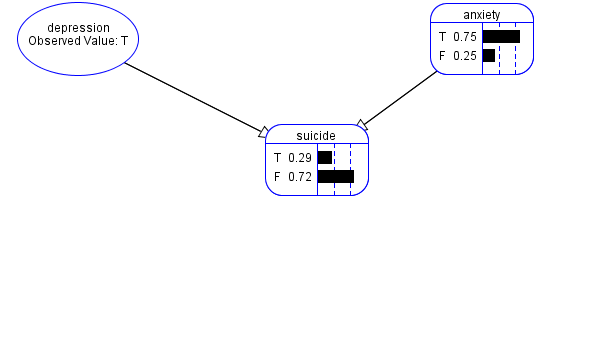
\includegraphics[scale=0.8]{ex111}
\end{center}

\tab Formulas and probability calculated:\\
\tab\tab p(s) = p(s/depr,anx) * p(dep) * p(anx) + p(s/depr,-anx) * p (depr) * p(-anx) =\\
\tab\tab = 0.3 * 1 * 0.2 + 0.8 * 1 * 0.25 = 0.09 + 0.2 = 0.29\\

\tab \textbf{Conclusion}In the query shown up, we assumed that the person has depression and it might have a 75 per cent change
to have anxiety. There will be 29 per cent probability that the person will commit suicide.\\

\item{Second example}

\tab The probability of a person to have a car is the following. There is a 75 per cent change for a person
with driving license to have a car,15 percent if he/she dosen't. There is a 62 per cent of change of people to have a driving license if they are of
legal age,but some can aquirre with the prob of 0.01 per cent a fals driving license, even thou they are not of legal age. 
\footnote{https://math.stackexchange.com/questions/408082/conditional-probability-question-about-students-owning-cars-and-bikes}

\begin{center}
  	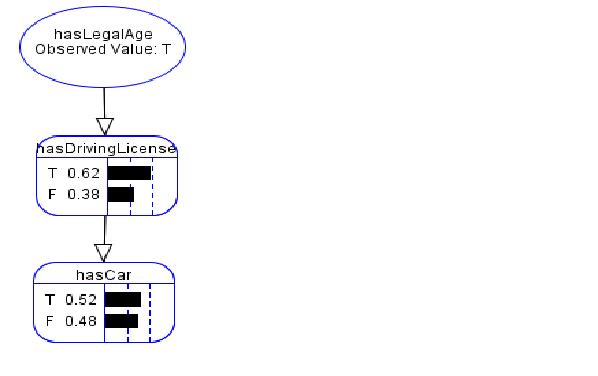
\includegraphics[scale=0.8]{ex22}
\end{center}

\begin{center}
  	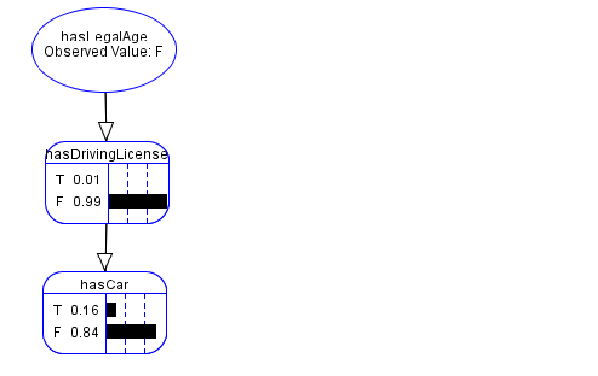
\includegraphics[scale=0.8]{ex222}
\end{center}


\tab \textbf{Conclusion} If we asume that the person has legal age , we see that there is a 52 per cent probability of a person to have a car.If the person is not legal aged there is a 16 per cent probability of having a car.\\


\item{Third example}

\tab The probability of hitting a person is given by the probability of having a car accident,  which is given by the brakes fails 25 per cent, driver fault 36 per cent. Not having breaks and dirver fault still puts a random person in danger by 3 per cent.If car is having an accident there is a 60 per cent prob of hitting a person, if it isn't there is only .001 per cent.\\

\begin{center}
  	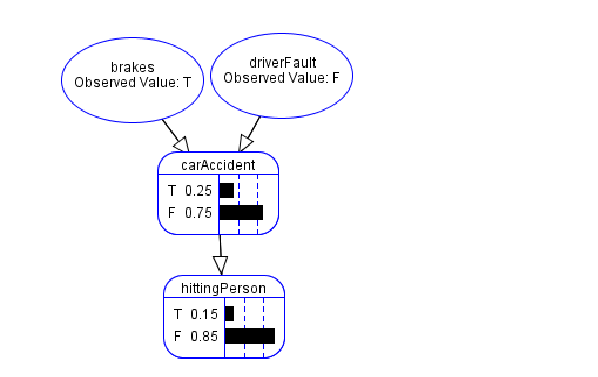
\includegraphics[scale=0.8]{ex33}
\end{center}

\begin{center}
  	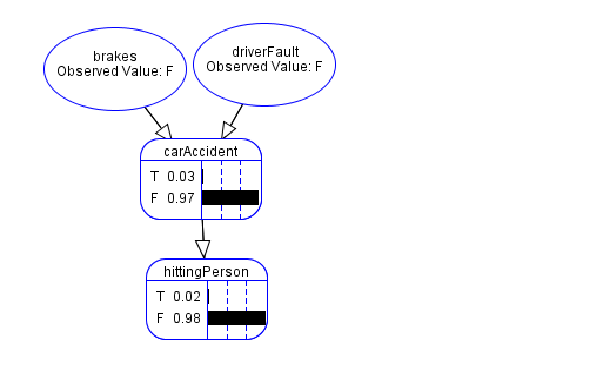
\includegraphics[scale=0.8]{ex333}
\end{center}


\tab \textbf{Conclusion} If we assume that the brake missfunctioned but driver didn't made any more faults, there is a 15 per cent probability of hitting a person. But, if the breaks were ok and the drive didn't make a mistake, there is a 2 per cent probability of hitting a person.\\

\item{Fourth example}\\
\tab The probability of getting fit will depend on the probability of hitting the gym(60) and the probability of being healthy(75). Being healthy will depend on how much healthy you eat(80) and how much sleep you get(60 ps)\\

\begin{center}
  	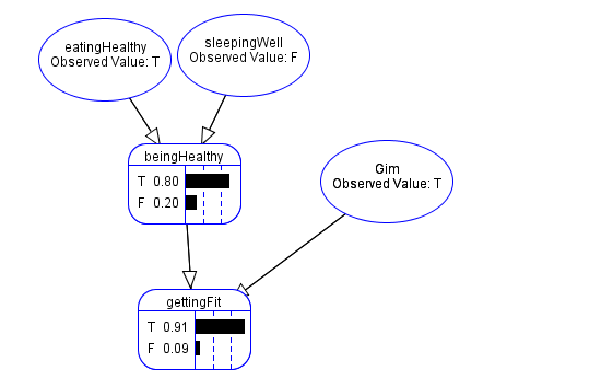
\includegraphics[scale=0.8]{ex4}
\end{center}

\begin{center}
  	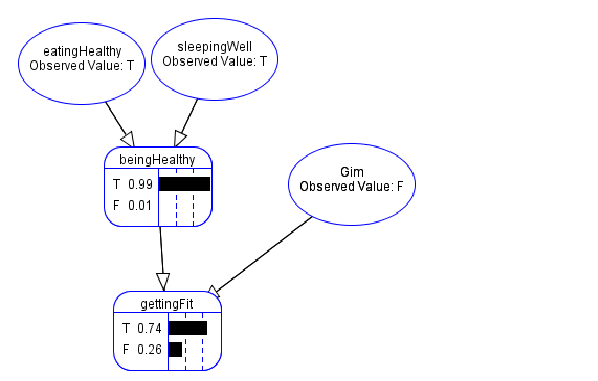
\includegraphics[scale=0.8]{ex44}
\end{center}


\tab \textbf{Conclusion} If we asume that the person will eat healthy but he won't be sleeping well. The person will go to the gym. There is a 91 probability of him getting fit.But if he eats healthy and sleeps well , but dosen;t go to the gim , he will have a 74 per cent change of getting fit.
\end{itemize}